\section{Experiments}
\label{sec:exp}

In this section, we conduct experiments to
(1) examine the performance of our PsyEx model compared with strong MDD baselines; (2) validate the effectiveness of multi-task learning and the proposed experts layer with ablation tests; (3) analyze the symptom contribution for the detection of each disease with interpretability enabled by PsyEx.

\begin{table*}[h]
    \small
    \centering
    \begin{tabular}{l|ccccccc|c}
    \hline
    Method & ADHD & Anxiety & Bipolar & Depression & Eating & OCD & PTSD & Mean \\ 
    \hline
    TF-IDF+LR & 59.55&	66.48&	66.67&	68.95&	11.11&	26.09&	30.43&	47.04\\
    BERT \citep{nguyen2022improving} & 60.05&	71.08&	43.56&	71.58&	37.04&	44.83&	27.45&	50.80\\
    Symp \citep{Zhang2022SymptomIF} & 60.14&	71.82&	67.76&	66.67&	52.17&	48.33&	48.48&	59.34 \\
    \hline
    PsyEx & \textbf{74.89}&    \textbf{77.97}&	\textbf{79.35}&	\textbf{79.62}&	\textbf{61.11} &	\textbf{61.84}&	\textbf{59.52}&	\textbf{70.61} \\ 
    %  -multi-attn & 73.33&	77.70&	78.32&	78.25&	46.67&	61.22&	61.33&	68.12 \\
    %  \hline
    % PsyEx (sum) &\textbf{75.17}& 	\textbf{79.45}&	\textbf{80.41}&	\textbf{79.80}&	\textbf{55.17}&	\textbf{67.61}&	\textbf{65.75}&	\textbf{71.91} \\
    %  -multi-attn & 70.43&	76.69&	78.85&	76.83&	56.25&	63.95&	63.16&	69.45 \\
    \hline
    \end{tabular}
    \caption{Mental Disease Detection Results across 7 diseases, reporting F1 scores.  }
    \label{tab:disease}
\end{table*}
% \MYW{Bold your best results for readability, explain the metrics and (max) in the table caption}

\begin{figure*}[th]
    \centering
    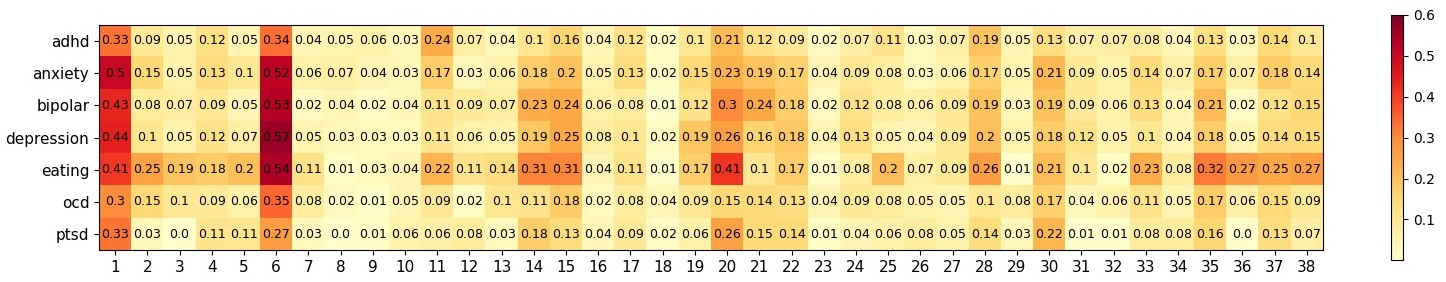
\includegraphics[width=\linewidth]{figures/symp_contribution_top1_full_symp_wo_dsm.jpg}
    \caption{Symptom contributions for MDD according to the attention scores obtain from 7 psychiatric "experts". 
    % \KZ{Make the fonts bigger in this fig. They are hardly legible. You can narrow the white space between the table and the right-most legend bar.}  
    We provide the corresponding symptom names with symptom id in Table \ref{tab:symp_id}, Appendix \ref{apd:symp_contribution}.}
    \label{fig:symp_contribution}
\end{figure*}

\subsection{MDD dataset}
\label{sec:mdd_dataset}
We use the MDD dataset constructed in \citet{Zhang2022SymptomIF}, which consists of 5,624 diagnosed users and 20,981 control users. Each diagnosed user can have one or more disease labels. We will train and evaluate the detection of each disease in a binary setting, and reported the average F1 score across all 7 diseases studied in this work. We provide the distribution of each disease in Appendix \ref{apd:stats}.
% 要注明我们只做了其中7种疾病的检测,去掉了精神分裂和Autism的疾病标签
% \MYW{You have to list out the full 7 diseases somewhere in the main text, by far I only see their types in Table 1, and better include their simple definition in the appendix}
Similar to SMHD \cite{cohan2018smhd}, this MDD dataset identifies mental disease patients by self-reported diagnostic patterns, like "I am diagnosed with".
Control users (non-patients) are randomly sampled from those who never posted or commented in mental health related subreddits. This dataset removes all the diagnostic posts but retains those mental health related posts to allow the extraction of symptom-related features. 

\subsection{Methods of Comparison}

For the MDD task, we mainly compared the proposed methods with 3 types of baselines: \textbf{TF-IDF+LR} is a representative traditional machine learning method which utilizes TF-IDF to extract textual features, followed by a Logistic Regression model for prediction. \textbf{BERT} is the reimplementation of the MDD model in \citet{nguyen2022improving}, which utilizes CNN of various kernel sizes on top of the sentence embeddings from pre-trained BERT as features to aggregate the information from users' posting list. \textbf{Symp} \cite{Zhang2022SymptomIF} further replace the features with symptoms features. Both of them establish strong baselines, especially \textit{Symp}. More details like hyperparameter settings can be found in Appendix \ref{apd:settings}.

\subsection{Experiment Results}

The MDD results are shown in Table \ref{tab:disease}. We can see that our proposed \textit{PsyEx} outperforms all the  baseline methods including the strong \textit{Symp} model, suggesting the advantage of our symptom-based risky post screening and psychiatric expert model in MDD. Further, owing to the multi-task learning and the shared knowledge between diseases, the detection effect of rarer classes (i.e. eating disorder, OCD, PTSD) is largely improved.

\begin{table}[h]
    % \small
    \centering
    \begin{tabular}{l|c}
        \hline
        Method & Avg. F1             \\
        \hline
        PsyEx &  70.61      \\
        ~~~~-multi-attn & 68.12       \\
        ~~~~-multi-task & 62.82     \\
        ~~~~-symp-risky & 50.68     \\
        % \hline
        % -multi-attn & Sum   & 69.45 \\
        \hline
    \end{tabular}
    \caption{Ablation tests for design choices of PsyEx, reporting F1 score averaged across 7 diseases. }
    \label{tab:ablation}
\end{table}

Moreover, we also examined the effectiveness of various design choices of the proposed PsyEx model with ablation tests in Table \ref{tab:ablation}.
First, we examine the $D$ disease-specific attention layers in PsyEx by implementing a similar model \textbf{-multi-attn}, in which all the diseases share a single attention head but are still trained simultaneously with multi-task learning. We can see that the performance is greatly harmed without multi-attention layer. 
Moreover, the \textbf{-multi-task} method further trains a \textit{-multi-attn} model for each disease and aggregate the performance of 7 models. The significant gap validated the necessity of multi-task learning, especially for rarer diseases. For example, we cannot even make a single correct prediction for \textit{eating disorder} without multi-task learning, potentially due to lack of positive samples (See detailed results in Table \ref{tab:mdd_by_disease}, Appendix \ref{apd:abl_results}). 
We also implement \textbf{-symp-risky}, which simply selects the \textit{last} $K$ post as risky posts, and its poor result demonstrates the importance of precise post screening methods.


% \MYW{This paragraph should be re-organized, introduce different methods with a special font or a bullet list}

\subsection{MDD Symptom Interpretation}
\label{sec:interpret}
% \MYW{Make it clear in the beginning that this section is for interpretations, the symptom contribution is actually a way to explain why the model makes the decision}

To explore the interpretability in the decision-making process of PsyEx, we measure the contribution of each symptom to the detection of different diseases, with the help of disease-specific experts in the model and selected risky posts. 

We apply the trained PsyEx model to diagnosed users in the test set, and get corresponding attention scores of his/her all risky posts.
For each user with disease $d$, we only select the post with highest attention score, and add its symptom probability to the symptom contribution vector. 
Finally, we normalized the symptom contribution vectors by dividing the number of users with each disease, and demonstrate them in a heat map (Figure \ref{fig:symp_contribution}) for all the diseases\footnote{We also provide another heat map (Figure \ref{fig:symp_contribution_wo_attn}) calculated without the assistance of attention score in Appendix \ref{apd:symp_contribution}.}.
% Here, we use serial numbers to represent symptoms, and provide the corresponding symptom names in Table \ref{tab:symp_id} (Appendix \ref{apd:symp_contribution}). 

In Figure \ref{fig:symp_contribution}, we can work out which symptoms are more critical for diagnosing a certain disease. The typical symptom "6: depressed mood"\footnote{We present the symptoms in "ID: name" format.} of depression, "1: anxious mood" of anxiety, and "11: Inattention" of ADHD exactly contributes more to the detection of them than to other diseases, which is in line with DSM-5 criteria\footnote{We provide the symptoms of 7 mental disorders (Table \ref{tab:symp_of_dsm5}) extracted from DSM-5 in Appendix \ref{apd:symp_contribution} for reference.}. 
Interestingly, we also find a few symptom-disease links supplementing the criteria, such as eating disorder patients are ``28: more talkative'' and tend to ``20: do things that easily get painful consequences'', both of which are typical symptoms for bipolar disorder, probably due to the high comorbidity of these two disorders proved by previous researches \cite{LUNDE2009relation, Ruiz2015Comorbidity}.
% \KZ{Rephrase this: ``do things easily get painful consequences''}, 
% \KZ{Is this a userful discovery?}
% \MYW{Consider making a figure containing posts along with disease prediction (multiple tags) and their corresponding symptoms}

% PsyEx suggests that "anxious mood", "depressed mood" is the most important symptoms for PSTD diagnosis, while "intrusion symptoms" and "avoidance of stimuli", two more PTSD-specific symptoms described in DSM-5, gets relatively lower attention in our model. That's probably because these two "mood" symptoms exists more common in the users' posts.  
